\documentclass{article}

\PassOptionsToPackage{numbers,compress}{natbib}
\usepackage[dblblindworkshop]{neurips_2026}
\workshoptitle{The Third Workshop on Agents in the Wild: Safety, Security, and Beyond}

\usepackage[utf8]{inputenc}
\usepackage[T1]{fontenc}
\usepackage{hyperref}
\usepackage{url}
\usepackage{booktabs}
\usepackage{amsfonts}
\usepackage{amsmath}
\usepackage{amssymb}
\usepackage{microtype}
\usepackage{graphicx}
\usepackage{xcolor}
\usepackage{tikz}
\usetikzlibrary{arrows.meta,positioning,fit,calc}

\title{Persistent Runtime Brakes for Multi-Agent Coordination}

\author{%
  Anonymous Author(s) \\
  Anonymous Institution
}

\begin{document}

\maketitle

\begin{abstract}
Agent frameworks can plan and protocols can move messages, but neither answers a prior question at the execution boundary: \emph{may this coordination step run, and does a refusal still bind after the request ends?}
We argue that many multi-agent failures are physical before they are semantic---stacked delegation can exhaust a node while every hop remains well-formed.
This short paper specifies a \emph{consequence persistence layer} (CPL): an out-of-band gate that adjudicates \emph{before} irreversible intent, stores allow~/delay~/isolate on identity, and can wrap an existing planner runtime.
On a LangGraph planner that issues real tool I/O (local lookup and HTTP GET) through a sidecar pre-flight path, a one-tool job and an eight-tool job both complete with or without the gate (false isolate $=0$); unbounded \texttt{tick} stacking reaches a 40-step cap without the gate and is isolated at depth 11 with it; a 48-task burst is refused at entropy $0.96$.
The reported table uses a deterministic tool-calling policy so the trial cannot flake; the same graph accepts a live OpenAI-compatible chat model.
A synthetic mesh in the appendix is a sanity check, not the main result: there, $100\%$ survival is an invariant of refusing increments past $0.95$ when death is load $\ge 1$.
CPL is a translation of admission control and circuit breaking onto agent trajectories, not a replacement for prompt-injection defense.
\end{abstract}

\section{Introduction}
\label{sec:intro}

Deployed agents now decompose work, call tools, and talk to other agents~\cite{yao2023react,wu2023autogen,langchain2025langgraph,anthropic2024mcp,google2025a2a}.
Safety research has followed the new attack surface: indirect prompt injection, tool misuse, and computer-use compromise~\cite{greshake2023not,debenedetti2024agentdojo,andriushchenko2024agentharm,hou2025mcp}.
A complementary failure mode is less discussed and already routine in multi-agent stacks.
A planner fans out into $A\!\rightarrow\!B\!\rightarrow\!C$, sometimes closing a loop.
Each hop can be a valid tool call or a polite protocol session.
The \emph{trajectory} still becomes physically unsustainable: recursion depth, context volume, concurrency, and neighbor load grow until the node saturates.

Per-request gateways forget.
Token budgets account after commit.
Framework \texttt{max\_retries} counters reset when the session ends, and they cannot see a chain that crosses process or host boundaries~\cite{cemri2025why}.
In-process guardrails share the optimizer's address space and cannot be attested to a distrusting peer.
Semantic protocols such as MCP and A2A~\cite{anthropic2024mcp,google2025a2a} decide \emph{what} may be said; they are not brakes on \emph{whether} the next optimization step may execute.

We call the missing object a \textbf{consequence persistence layer} (CPL).
CPL sits at the execution boundary---the narrow interface where planning, delegation, and I/O meet compute, memory, and the wire---and enforces three contracts:
(i)~adjudicate \emph{before} irreversible intent or ingress;
(ii)~bind the verdict to an agent or peer identity so it survives the request;
(iii)~use one authority for governing the local planner and admitting foreign traffic.

This is a short paper, not a claim that CPL replaces alignment, sandboxing, or injection defense.
The braking primitive is old: admission control, backpressure, and circuit breakers are standard in production systems~\cite{nygard2018release,fowler2014circuit,jacobson1988congestion,welsh2001seda,netflix2012hystrix,envoy2024circuit}.
What is missing in agent stacks is applying that primitive \emph{before} a planner hop, on \emph{agent identity}, with one authority for local generation and foreign ingress.

Our contributions are:
\begin{enumerate}
    \item a layer diagnosis: planning and transport are populated; runtime coordination law is not;
    \item a compact dual-path protocol that wraps existing planner nodes rather than replacing the framework;
    \item a paired LangGraph tool trace (gate on vs.\ off), including completion and false-isolate columns, plus an explicit statement that a prior mesh simulation is a model invariant, not field evidence.
\end{enumerate}

\section{A consequence persistence layer}
\label{sec:method}

\paragraph{Dual path, one authority.}
A node faces two ingresses that must not split-brain.
\emph{Path~A} (govern self) is a synchronous pre-flight probe from the local planner \emph{before} it emits a tool call, delegation, or outbound message.
\emph{Path~B} (govern neighbors) validates a physical \emph{governance header} \emph{before} any business payload is admitted.
Both paths query the same \textbf{single execution authority} (SEA): one policy snapshot, one pressure monitor, one state machine.
If Path~A were strict and Path~B lax, a locally throttled planner could still flood peers; the reverse lets inbound work overwhelm a node that has already stopped its own optimizer.

\paragraph{What is judged.}
SEA does not parse natural language, tool schemas, or session text.
It evaluates a physical bundle: system pressure $e\in[0,1]$, planner recursion depth, a burst hint (estimated imminent fan-out), and a peer viability score $v\in[0,1]$.
Reference pressure is a max-pool of normalized tool concurrency, memory, context volume, and burst:
\begin{equation}
    e \;=\; \max\!\bigl(e_{\mathrm{tool}},\, e_{\mathrm{mem}},\, e_{\mathrm{ctx}},\, e_{\mathrm{burst}}\bigr).
    \label{eq:entropy}
\end{equation}
Catastrophe is limited by the worst axis, not the average.
Bands in the reference policy are $e_{\mathrm{safe}}=0.40$, $e_{\mathrm{warn}}=0.75$, and a hard limit $e^{\star}=0.95$.
Crossing $e^{\star}$ or a configured depth cap isolates immediately.

\paragraph{Consequences persist.}
Every probe returns one letter from a closed alphabet: \textsc{allow}, \textsc{delay}$(\delta)$, or \textsc{isolate}.
There is no advisory mode.
The letter is stored on identity, not on request id, and remains in force across scheduling epochs until a recovery rule fires.
A four-state machine implements asymmetric hysteresis: \textsc{permissive} $\leftrightarrow$ \textsc{throttled} on pressure bands; \textsc{isolated} after a signature failure, a malicious spike, or $v<v_{\mathrm{crit}}$; \textsc{probationary} only after a long dwell.
Recovery is slow by construction (reference: 64 epochs isolated, 128 on probation, and $v\ge 0.8$ to return to full egress).
Request completion does \emph{not} clear isolation.

\paragraph{Open meshes (specified, not evaluated here).}
Inside an administrative boundary, Path~A is the primary brake.
Path~B and a local viability score $v\in[0,1]$ are specified for strangers and hit-and-run peers (Appendix~\ref{app:cvp}); this paper's runtime trace uses Path~A only.
Identity-persisted penalties can be evaded by minting a fresh identity---an open-mesh limitation we do not claim to close.

\paragraph{Placement.}
CPL is out-of-band: it must not depend on the application protocol cooperating.
A reference implementation exposes pre-flight as local IPC and wraps planner nodes in graph-based agent frameworks so a blocked step can halt or annotate state instead of throwing the process into an ungoverned retry storm.
Enterprise and open-mesh deployments share the same kernel; only the trust posture on Path~B changes.

\begin{figure}[t]
\centering
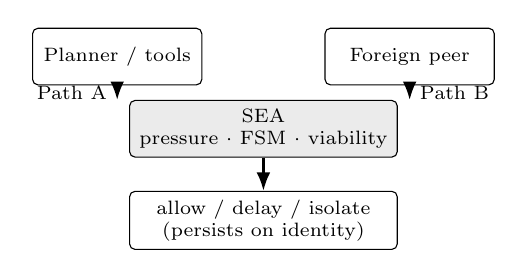
\begin{tikzpicture}[
  font=\scriptsize,
  box/.style={draw, rounded corners=2pt, align=center, inner sep=3pt, minimum height=0.72cm},
  sea/.style={box, fill=black!8, minimum width=3.4cm},
  path/.style={box, fill=white, minimum width=2.15cm},
  arr/.style={-{Latex}, thick}
]
\node[path] (plan) {Planner / tools};
\node[path, right=1.55cm of plan] (peer) {Foreign peer};
\node[sea, below=0.55cm of $(plan)!0.5!(peer)$] (sea) {SEA \\ pressure $\cdot$ FSM $\cdot$ viability};
\node[box, fill=white, below=0.42cm of sea, minimum width=3.4cm] (cons) {allow / delay / isolate \\ (persists on identity)};
\draw[arr] (plan) -- node[left, font=\scriptsize] {Path A} (sea.north -| plan);
\draw[arr] (peer) -- node[right, font=\scriptsize] {Path B} (sea.north -| peer);
\draw[arr] (sea) -- (cons);
\end{tikzpicture}
\caption{CPL in one picture. Path~A brakes the local optimizer before intent leaves; Path~B brakes neighbors before payload admission. Both share one authority and one persistent consequence.}
\label{fig:arch}
\end{figure}

\section{A planner-tool trace}
\label{sec:exp}

We evaluate Path~A on a LangGraph that calls tools: a local key lookup and HTTP GET against a loopback fixture.
Pre-flight sits \emph{before} the tool runs, not after the planner talks.
The reported table uses a deterministic tool-calling policy so stacking and burst cannot flake; the same graph speaks OpenAI-compatible \texttt{/v1/chat/completions}.
A local Qwen2.5 0.5B completes S1 in both modes (false isolate $=0$); it does not finish the eight-tool S2 recipe, and a looping live planner is isolated at the recursion cap (Appendix~\ref{app:persist}).
The question is whether pre-flight changes \emph{this} trajectory, and whether legitimate jobs still finish.

\paragraph{Paired modes.}
The graph is identical.
\emph{Off:} planner and tools always run; the only stop is a graph depth cap.
\emph{On:} each planner hop and each tool call reports depth and context bytes, then blocks on pre-flight; isolate annotates state and stops the graph.
Sidecar policy uses the reference recursion cap ($10$) and concurrency cap ($50$).

\paragraph{Jobs.}
\emph{S1} one lookup.
\emph{S2} eight hops (four lookups, four GETs)---longer than S1, still under the depth cap.
\emph{S3} graph-driven \texttt{tick} stacking to a cap of $40$.
\emph{S4} one \texttt{expand} with burst hint $48$ (entropy $48/50=0.96$), then queued GETs if allowed.

\begin{table}[t]
\caption{Paired Path~A traces on real tool I/O. S1/S2 complete in both modes (false isolate $=0$). S3/S4 run to completion without the gate and are isolated with it.}
\label{tab:trace}
\centering
\setlength{\tabcolsep}{2.6pt}
{\scriptsize
\begin{tabular}{llcccccl}
\toprule
Job & Gate & Done & Tools & Probes & Isolated & Depth & Reason \\
\midrule
S1 short & off & yes & 1 & 0 & no & 2 & --- \\
S1 short & on & yes & 1 & 3 & no & 2 & --- \\
S2 long & off & yes & 8 & 0 & no & 9 & --- \\
S2 long & on & yes & 8 & 17 & no & 9 & --- \\
S3 runaway & off & to cap & 39 & 0 & no & 40 & --- \\
S3 runaway & on & no & 10 & 22 & yes & 11 & recursion cap \\
S4 storm & off & yes & 49 & 0 & no & 50 & --- \\
S4 storm & on & no & 0 & 2 & yes & 1 & burst entropy \\
\bottomrule
\end{tabular}
}
\end{table}

\paragraph{Reading Table~\ref{tab:trace}.}
S1 and S2 finish with the gate on: the eight-tool job is the false-isolate check the one-hop job does not cover.
S3 without the gate walks to the graph cap (depth $40$, $39$ ticks); with it, isolation fires at reported depth $11$ after $11$ planner steps.
S4 without the gate performs the expand plus $48$ GETs; with it, the burst hint opens the breaker at entropy $0.96$ and no GET runs.
Wall-clock on these runs is tens of milliseconds; we do not treat that as a load test.

This is not computer-use, MCP ingress, or prompt-injection robustness.
It is pre-flight on an actual planner graph with real tool I/O, a completion column, and a long-enough benign job.

\paragraph{What we still do not claim.}
Path~B, viability, stranger tax, and gossip are unspecified by this table.
An open-mesh adversary who rotates identities can evade identity-persisted penalties.
Throughput under mixed production models, and MCP \emph{ingress}, remain open.
A leftover high recursion depth still isolates a later probe on the same sidecar; a new graph that reports depth $0$ is admitted---Path~A currently persists last telemetry, not a dwell-locked letter (Appendix~\ref{app:persist}).
On the S1--S4 jobs a per-step gate that wipes leftover state matches the current sidecar; they split only on a stale post-isolate probe (Appendix~\ref{app:baseline}).

\section{Related work}
\label{sec:related}

\paragraph{Admission control and circuit breaking.}
Refusing work before overload is standard operations practice: TCP congestion control~\cite{jacobson1988congestion}, staged event-driven backpressure~\cite{welsh2001seda}, the circuit-breaker pattern~\cite{nygard2018release,fowler2014circuit}, and production proxies such as Hystrix and Envoy~\cite{netflix2012hystrix,envoy2024circuit}.
CPL does not invent that primitive.
It attaches it to \emph{optimizer trajectories}: a verdict that is pre-intent, bound to agent identity rather than to one RPC, and shared by local planner hops and (in the spec) neighbor ingress.
Framework \texttt{max\_retries} and token budgets remain necessary telemetry; they still reset per session or account after commit~\cite{cemri2025why}.

\paragraph{Agent frameworks} decompose and converse~\cite{yao2023react,wu2023autogen,hong2023metagpt,li2023camel,langchain2025langgraph,crewai2025,park2023generative,shinn2023reflexion}.
They optimize task completion, not a persistent execution-boundary brake.

\paragraph{Agent safety evaluations} measure harmfulness, injection, and tool abuse~\cite{debenedetti2024agentdojo,andriushchenko2024agentharm,ruan2024identifying,greshake2023not}.
Those tests grade speech and tool policy.
They do not ask whether a well-formed graph can still saturate its host.

\paragraph{Control and oversight.}
AI control~\cite{greenblatt2024control}, debate~\cite{irving2018debate}, constitutional feedback~\cite{bai2022constitutional}, scalable oversight~\cite{kenton2024oversight}, and representation-level circuit breakers~\cite{zou2024circuit} constrain \emph{intent}.
CPL constrains \emph{capacity at the boundary}.
A monitored but unbraked fleet can still loop itself into unavailability.

\paragraph{Agent protocols.}
MCP and A2A~\cite{anthropic2024mcp,google2025a2a,hou2025mcp} secure tools and sessions.
A valid MCP call can still be a physically illegal next hop.
The layers compose: policy and injection defense first; CPL second.

\section{Discussion}
\label{sec:disc}

What we claim: multi-agent stacks need a pre-intent brake on physical trajectories; Path~A can wrap a LangGraph node and its tools, stop a recursion runaway and a burst that the same graph otherwise runs to completion, and still finish a short and an eight-tool job.
What we do not claim: that the mesh simulation proves field safety; that viability or Path~B is empirically necessary; that CPL replaces injection defense, sandboxing, or human oversight; or that identity persistence survives an identity-budget attack.

The remaining gap is ingress, mixed hosted-model traffic, and a verdict that survives a healthy rewrite of host telemetry rather than leftover depth.
Until those exist, CPL is a specified brake with a planner-tool trace---not a completed in-the-wild safety result.

\clearpage
\bibliography{references}
\bibliographystyle{plainnat}

\appendix
\section{Supplementary material}
\label{app:supp}

This appendix does not count toward a short-paper page limit.
It records a depth-only graph check, a three-way baseline, cross-request telemetry, two local planners, the synthetic mesh as a \emph{sanity check}, Path~B viability (specified, not traced), and an implementation sketch.

\subsection{Synthetic depth-only graph}
\label{app:synth-depth}

Before tools were wired, the same sidecar isolated a depth-only planner (no lookup, no HTTP) at the recursion cap.
Table~\ref{tab:synth-depth} is that check; Table~\ref{tab:trace} is the main result.

\begin{table}[h]
\centering
\caption{Depth-only LangGraph (no tool I/O). Kept as a unit check, not as the main evidence.}
\label{tab:synth-depth}
\centering
\setlength{\tabcolsep}{3.2pt}
{\scriptsize
\begin{tabular}{llcccccl}
\toprule
Job & Gate & Finished & Steps & Probes & Isolated & Depth & Reason \\
\midrule
Benign & off & yes & 3 & 0 & no & 3 & --- \\
Benign & on & yes & 3 & 3 & no & 3 & --- \\
Runaway & off & to cap & 40 & 0 & no & 40 & --- \\
Runaway & on & no & 11 & 12 & yes & 11 & recursion cap \\
\bottomrule
\end{tabular}
}
\end{table}

\subsection{Persistence and two local planners}
\label{app:persist}

Path~A isolation follows last-reported host telemetry on one sidecar, not a dwell-locked letter on agent identity.
After S3 isolates, a later probe that does \emph{not} rewrite depth is still refused; a new S1 graph that reports depth $0$ is admitted (Table~\ref{tab:persist}).
Two planners on \emph{separate} sidecars do not share that monitor: A can isolate while B still completes S1.
On one shared sidecar, B's fresh report overwrites A's leftover depth (Table~\ref{tab:two}).

\begin{table}[h]
\centering
\caption{Same sidecar after S3 isolate. Stale probe keeps the leftover depth; a new S1 overwrites it.}
\label{tab:persist}
{\scriptsize
\begin{tabular}{lccc}
\toprule
Arm & Isolated & S1 done & Reason \\
\midrule
Stale probe (no rewrite) & yes & --- & recursion cap \\
Fresh S1 (reports depth $0$) & no & yes & --- \\
\bottomrule
\end{tabular}
}
\end{table}

\begin{table}[h]
\centering
\caption{Two local planners. Split sidecars keep B healthy; a shared sidecar lets B overwrite A's telemetry.}
\label{tab:two}
{\scriptsize
\begin{tabular}{llccc}
\toprule
Layout & Agent & Job & Isolated & Done \\
\midrule
Split sidecars & A & S3 & yes & no \\
Split sidecars & B & S1 & no & yes \\
Shared sidecar & A & S3 & yes & no \\
Shared sidecar & B & S1 & no & yes \\
\bottomrule
\end{tabular}
}
\end{table}

A local Qwen2.5 0.5B via OpenAI-compatible \texttt{/v1/chat/completions} completes S1 with and without the gate.
It does not execute the eight-tool S2 recipe: without the gate the graph hits its recursion limit; with the gate a looping live planner is isolated at depth $11$ (Table~\ref{tab:live}).
That is a model-quality result, not a false-isolate of a finished job.

\begin{table}[h]
\centering
\caption{Live Path~A on Qwen2.5 0.5B. S1 is the only completed live job.}
\label{tab:live}
{\scriptsize
\begin{tabular}{llcccc}
\toprule
Job & Gate & Done & Tools & Isolated & Reason \\
\midrule
S1 short & off & yes & 1 & no & --- \\
S1 short & on & yes & 1 & no & --- \\
S2 long & off & no & 0 & no & graph cap \\
S2 long & on & no & 10 & yes & recursion cap \\
\bottomrule
\end{tabular}
}
\end{table}

\subsection{No gate, stateless per-step, current sidecar}
\label{app:baseline}

Table~\ref{tab:baseline} compares three gates on the same scripted planner and tools.
\emph{Off} has no pre-flight.
\emph{Stateless} uses the same sidecar checks but reports depth $0$ at the start of each request, wiping leftover telemetry.
\emph{AFP} is the current sidecar: leftover depth is kept.
Five bounded jobs complete under every gate (false isolate $=0$): S1, S2, lookups-only, fetches-only, and eight repeats of the same lookup.
S3 and S4 are contained by both gated columns and run to completion without a gate.
Mean wall-clock on the bounded jobs is $3.8$\,ms off and $6.0$--$6.4$\,ms gated; we do not treat that as a load test.

The gates diverge only after isolate.
A stale probe (no rewrite) is refused by AFP and admitted by the stateless wipe; a new S1 that reports depth $0$ completes under both.
So the incremental object relative to a per-step policy is leftover telemetry, not a dwell-locked identity letter.

\begin{table}[h]
\centering
\caption{Three-way baseline. Bounded jobs: $5/5$ complete, false isolate $=0$. Containment and the stale probe are the informative columns.}
\label{tab:baseline}
{\scriptsize
\begin{tabular}{lcccc}
\toprule
Gate & Bounded done & S3/S4 isolated & Stale probe & Fresh S1 \\
\midrule
Off & $5/5$ & $0/2$ & --- & --- \\
Stateless & $5/5$ & $2/2$ & allow & done \\
AFP & $5/5$ & $2/2$ & refuse & done \\
\bottomrule
\end{tabular}
}
\end{table}

\subsection{Synthetic mesh: an invariant, not a field result}
\label{app:mc}

Death is defined as load $\ge 1$.
The simulated gate refuses any request with $\mathrm{load}+\mathrm{request}>0.95$.
Under that pair of rules a node cannot die: $100\%$ survival is an invariant of the construction, not evidence about LLM agents.
We keep the numbers because they show the complementary fact: without any pre-accumulation refusal, the same seeds collapse (mean $1.88/500$ alive at $T=100$ over $1{,}000$ runs).
Ablations (Table~\ref{tab:ablate}) locate the invariant in the breaker, not in viability.

\begin{table}[h]
\centering
\caption{Mean survival (\%) at $T=100$. Breaker-only matches full CPL; viability-only matches baseline.}
\label{tab:ablate}
\centering
\setlength{\tabcolsep}{3.4pt}
{\scriptsize
\begin{tabular}{lcccccc}
\toprule
Malicious \% & Full & No $v$ floor & No breaker & No burst tax & Breaker only & $v$ only / base \\
\midrule
$5$  & $100$ & $100$ & $4.8$  & $100$ & $100$ & $0.3$ / $0.3$ \\
$20$ & $100$ & $100$ & $15.7$ & $100$ & $100$ & $0.2$ / $0.2$ \\
\bottomrule
\end{tabular}
}
\end{table}

\begin{figure}[h]
\centering
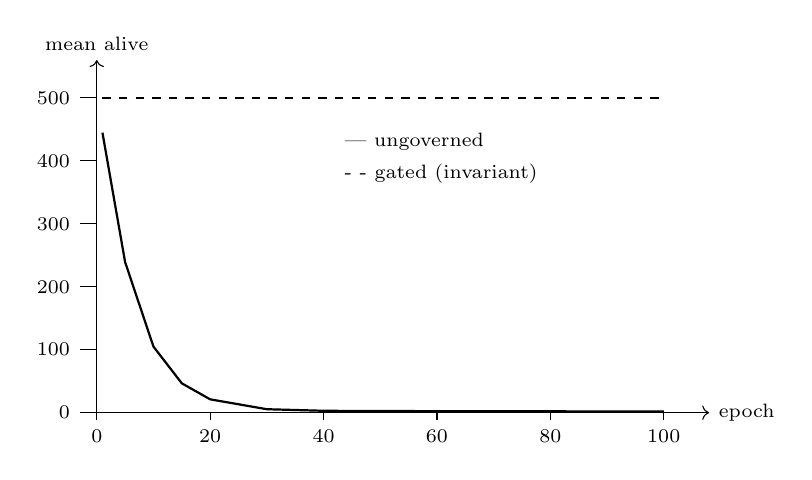
\begin{tikzpicture}[x=0.072cm,y=0.008cm, font=\scriptsize]
  \draw[->] (0,0) -- (108,0) node[right] {epoch};
  \draw[->] (0,0) -- (0,560) node[above] {mean alive};
  \foreach \x in {0,20,40,60,80,100}
    \draw (\x,0) -- (\x,-12) node[below] {\x};
  \foreach \y in {0,100,200,300,400,500}
    \draw (0,\y) -- (-3,\y) node[left] {\y};
  \draw[thick]
    (1,444.8) -- (5,239.1) -- (10,104.9) -- (15,46.6) -- (20,21.2)
    -- (30,5.5) -- (40,3.0) -- (50,2.6) -- (75,2.2) -- (100,1.9);
  \draw[thick, dashed] (1,500) -- (100,500);
  \node[anchor=west] at (42,430) {--- ungoverned};
  \node[anchor=west] at (42,380) {- - gated (invariant)};
\end{tikzpicture}
\caption{Mean alive nodes, $1{,}000$ paired runs ($N=500$, $5\%$ malicious). Treat as a model check, not a deployment result.}
\label{fig:curve}
\end{figure}

\subsection{Reference constants}
\label{app:const}

\begin{table}[h]
\centering
\caption{Kernel and mesh-sanity-check constants. Tool traces use sidecar recursion cap $10$, concurrency cap $50$, S2 $=8$ hops, S3 graph cap $40$, S4 burst hint $48$.}
\label{tab:const}
{\small
\begin{tabular}{ll}
\toprule
Symbol / name & Value \\
\midrule
$N$, epochs, runs (main curve) & $500$, $100$, $1{,}000$ \\
Runs (sweeps / ablations) & $300$ \\
Fan-out, cool-down & $3$ requests / node / epoch, $\times 0.5$ \\
Benign / malicious request load & $0.1$ / $0.8$ \\
Fatal load, breaker threshold $e^{\star}$ & $1.0$, $0.95$ \\
$v_{\mathrm{crit}}$, burst-tax threshold & $0.3$, $0.5$ \\
Breaker penalties (malicious / benign) & $-0.5$ / $-0.1$ \\
Burst-tax penalty & $-0.3$ \\
Eq.~\eqref{eq:cvp}: $\alpha$, $\beta$ & $0.95$, $0.05$ \\
Idle decay $\lambda$, recovery $\kappa$ & $0.01$ / epoch, $0.02$ \\
Isolation / probation dwell & $64$ / $128$ epochs \\
Permissive re-entry floor & $v \ge 0.8$ \\
Pressure bands $e_{\mathrm{safe}}$, $e_{\mathrm{warn}}$ & $0.40$, $0.75$ \\
\bottomrule
\end{tabular}
}
\end{table}

\subsection{Malicious-rate and fragmented-load sweeps}
\label{app:sweep}

The $100\%$ rows below are the same invariant as Figure~\ref{fig:curve}: the breaker refuses any increment that would cross $0.95$ before load can reach $1$.
They are not an independent empirical result.

\begin{table}[h]
\centering
\caption{Mean survival (\%) at $T=100$ vs.\ malicious fraction (300 runs).}
\label{tab:rate}
{\small
\begin{tabular}{lcccccccc}
\toprule
Mode & $1\%$ & $5\%$ & $10\%$ & $15\%$ & $20\%$ & $30\%$ & $40\%$ & $50\%$ \\
\midrule
Baseline & $2.3$ & $0.3$ & $0.3$ & $0.3$ & $0.2$ & $0.2$ & $0.2$ & $0.2$ \\
CPL (full) & $100$ & $100$ & $100$ & $100$ & $100$ & $100$ & $100$ & $100$ \\
\bottomrule
\end{tabular}
}
\end{table}

\begin{table}[h]
\centering
\caption{Mean survival (\%) when malicious per-request load is reduced (5\% malicious, 300 runs).}
\label{tab:adapt}
{\small
\begin{tabular}{lcccc}
\toprule
Malicious load & $0.80$ & $0.45$ & $0.20$ & $0.12$ \\
\midrule
Baseline & $0.3$ & $0.6$ & $3.1$ & $7.8$ \\
CPL (full) & $100$ & $100$ & $100$ & $100$ \\
\bottomrule
\end{tabular}
}
\end{table}

\subsection{Viability (specified; idle in the mesh check)}
\label{app:cvp}

For peer $p$ at node $n$, coordination viability $v_n(p)\in[0,1]$ is specified as
\begin{equation}
    v \;\leftarrow\; \mathrm{clip}_{[0,1]}\!\bigl(\alpha v + \beta\,\tau - \gamma\,d - \delta\,e\bigr),
    \label{eq:cvp}
\end{equation}
with $\alpha=0.95$, $\beta=0.05$.
In the mesh check, $v$ decreases only when the breaker or burst tax fires, so a viability-only policy never isolates.
Identity rotation can also reset $v$; Path~A on a local planner does not address that adversary.

\subsection{Why viability looks idle in the harness}
\label{app:why}

A viability-only policy never observes $v<v_{\mathrm{crit}}$ unless some other rule first writes a penalty; that is why ``$v$ only'' matches baseline in Table~\ref{tab:ablate}.
In the full protocol, $v$ is written by Path~B attestation failures, stranger-tax refusals, and gossiped isolation warnings---none of which the abstract harness models.
The correct reading is: \emph{local physical refusal is the survival mechanism against dumb exporters; viability is a mesh-memory mechanism awaiting a contagion / hit-and-run eval.}

\subsection{Implementation sketch (anonymized)}
\label{app:impl}

A conforming Path~A runtime:
\begin{enumerate}
    \item reports recursion depth and context bytes to the pressure monitor;
    \item issues a blocking pre-flight RPC with a burst hint;
    \item proceeds only on \textsc{allow}, sleeps $\delta$ on \textsc{delay}, and must not emit I/O on \textsc{isolate}.
\end{enumerate}
A conforming Path~B hop sends a length-prefixed governance header as frame~1 and treats the header as a claim to be re-measured.
Enterprise (closed) and open-exchange profiles share entropy, depth, and FSM law; the open profile adds collateral and header attestation.
Code and deployment names are withheld for double-blind review and can be restored in the camera-ready version.

\end{document}
